\chapter{Relativistic Momentum and Energy}
\label{chapter:relativity_pande}


%\section*{Objectives}
%\begin{objectives}
%\item Know the modifications in the definitions of momentum and energy
% needed to maintain invariance of the conservation laws.
%%\item Show that $E^2- p^2c^2$ is a constant, related to a particle's
%%mass and independent of velocity.  
%\item Given any two of a particle's dynamical quantities ($p$, $E$, $u$, $K$,
%and $m$) determine any of the others.  
%\item Specialize any of the equations relating $p$, $E$, $u$, $K$, and $m$ to
%zero-mass particles.
%\end{objectives}

\section{Introduction}

So far in our discussions of relativity, we have taken a very simple
principle --- the {\em Principle of Relativity}, which states that the
laws of physics are the same for observers in any inertial reference
frame --- and have used this principle to change completely our notions
of how time and space work.  But we are not yet done looking at the
implications of this principle.  It will be necessary to generalize
the classical relations for energy and momentum to account for the
strange behavior that we have already seen at relativistic velocities.
And the new relativistic equations for energy and momentum carry
significant implications that change our notions of energy and matter.
This discussion leads to what is probably the most famous equation in
all of physics --- namely $E = mc^2$ --- as well as the basic principle
behind nuclear power generation.  Of course, this is also the principle 
behind nuclear weapons, so it can be argued that this result fundamentally
changed society.  But this is also the principle behind energy generation
in stars (including our own Sun); there would be no life on this planet
without this principle.
% As we will see, we will also find a new invariant in this discussion;
% namely, the combination $E^2 - p^2c^2$.

But before we discuss relativistic energy and momentum, we will take
a closer look at the concept of velocity.  If observers in different
reference frames don't agree on the results of measurement of lengths 
and time intervals, they won't agree on the results of their determinations
of velocities. 


\section{Relativistic Velocity Transformations}

Let's say that two spaceships leave Earth.  The {\em USS Zaphod}
leaves the Earth going in one direction with a speed $0.8c$ relative
to Earth.  The {\em USS Beeblebrox} leaves Earth going in the opposite
direction with a speed $0.8c$ relative to Earth.  What is the speed
of the {\em Zaphod} from the reference frame of the {\em Beeblebrox}?
Based on classical assumptions, you might expect the answer to be
$1.6c$.  But this conflicts with Einstein's theory of relativity which
states that no object can travel faster than the speed of light
relative to any other observer.  It is clear that it is necessary to
replace classical laws for addition and subtraction of velocities with
a more general, relativistic transformation.

A relativistic approach to velocity addition and subtraction was already
hinted at earlier in Chapter \ref{chapter:relativityI}.  The principle
of invariance of the speed of light requires that all observers (in
any reference frame) measure the same speed for a pulse of light ---
we can't simply add and subtract velocities.  On the other hand, common
experience shows us that for non-relativistic speeds, simple addition
and subtraction work fine.  So, we need a velocity transformation
relation that reduces to the classical result for small speeds, but
which prevents anything from traveling faster than the speed of light.
It turns out that this can be accomplished by taking the classical result
and dividing by a relativistic correction that becomes significant (i.e.,
not just 1) for speeds close to $c$.

Figure \ref{fig:rel1_vtransform} shows the scenario that we are
discussing.  Two reference frames are defined: an unprimed frame
denoted by observer A and a primed frame denoted by observer B on a
spaceship moving with a speed $v$ relative to observer A.  They are both
measuring the speed of the same object.  Observer A says the object is
moving with a speed $u_{\rm obj}$ while observer B says the ball is
moving with a speed $u_{\rm obj}^\prime$.

\begin{figure}[tbp]
\begin{center}
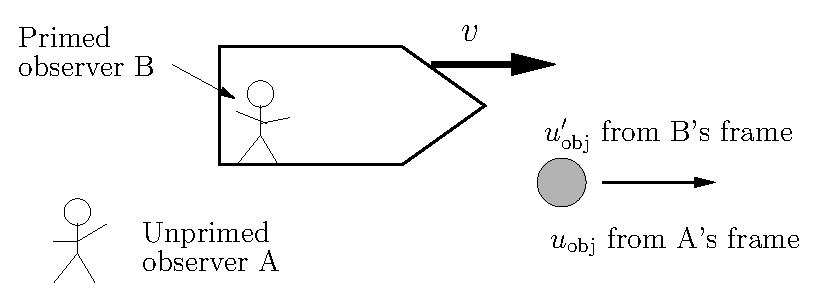
\includegraphics[width=4in]{basic_postulates_of_relativity/rel1_vtransform.eps}
\end{center}
\caption{An object moving in the $x$-direction relative to both
unprimed and primed frames.  The speed of the object is measured to be
$u_{\rm obj}$ from the reference frame of observer A and 
$u_{\rm obj}^\prime$ from the reference frame of observer~B.}
\label{fig:rel1_vtransform}
\end{figure}   

The question is: How are $u_{\rm obj}$, $u^\prime_{\rm obj}$ and $v$ related?
The answer is given by a {\em velocity transformation} equation,

\begin{boxiteq}
{\begin{equation}
u_{\rm obj} = \frac{u_{\rm obj}^\prime + v}{1 + u_{\rm obj}^\prime v/c^2}.
\label{eq:vtransform}
\end{equation}}
\end{boxiteq}
                                                
\noindent Equation (\ref{eq:vtransform}) is used to relate an object's
velocity in one frame to that as viewed in another frame.

We won't derive Eq.~(\ref{eq:vtransform}) rigorously here.  Rather,
note that if the object is a pulse of light, then $u_{\rm obj}^\prime
= c$, and Eq.~(\ref{eq:vtransform}) reduces to
\begin{equation}
u_{\rm obj} = \frac{c+v}{1 + cv/c^2} = \frac{c+v}{1+v/c} = 
c\left(\frac{c+v}{c+v}\right) = c.
\end{equation}
Both observers measure the object to have a speed $c$, so, the
invariance of the speed of light is preserved in this transformation.

Note that the numerator in Eq.~(\ref{eq:vtransform}) is the result
that you would get classically, whereas the denominator is a
relativistic correction. Also, note that if either the object or the
primed observer are traveling at speeds that aren't a significant
fraction of the speed of light, then the denominator of
Eq.~(\ref{eq:vtransform}) is very nearly 1, so we recover the
classical result for ``everyday'' speeds.
    
We'll show how to work with this relation in the next example.

\begin{example}{Baseball velocity addition}
  Bucknell Bison baseball pitcher Christy Mathewson throws a blazing 
  fastball while riding on a really fast train.
  From his reference frame (i.e., the train's frame) the ball moves
  toward the front of the train with a speed $u_{\rm ball} = 0.7c$.
  The train itself is moving relative to the ground with speed $v =
  0.8c$.  How fast is the ball moving relative to someone on the
  ground?  

\solution Classically, the speed as viewed from the ground
  would be $u_{\rm ball} + v$ or $1.5c$.  (This is the numerator of
  Eq.~(\ref{eq:vtransform}).)  But, of course, this isn't possible in
  a relativistic universe where nothing goes faster than $c$.  Using
  Eq.~(\ref{eq:vtransform}) we find
\begin{equation}
  u_{\rm ball} = \frac{u_{\rm ball}^\prime + v}{1+ u_{\rm ball}^\prime v/c^2}
  = \frac{0.7c + 0.8c}{1+0.7\times 0.8} = 0.96c.
\end{equation}
Note that relativistic correction keeps the speed less than $c$.

\noindent {\bf Exercise}: What if the ball were a beam of light?  How
fast would it be moving from the train's reference frame?  How fast
from the ground's reference frame?  Show that
Eq.~(\ref{eq:vtransform}) gives the correct result for this case.
\end{example}

If the problem gives you the speed as measured by the unprimed observer, 
you can use the following inverse transformations to get the speed as
measured by the primed observer:

\begin{boxiteq}
{
\begin{equation}
u_{\rm obj}^\prime = \frac{u_{\rm obj}- v}{1 - u_{\rm obj} v/c^2}.
\label{eq:vtransform-inverse}
\end{equation}
}
\end{boxiteq} 

You don't really need to write down these relations or try to figure
out which speed is $v$, which speed is $u_{\rm obj}$, and which speed
is $u_{\rm obj}^\prime$.  There is a very simple way of handling all
of these problems.  No matter which velocity you are looking for, the
answer is always:
\begin{equation}
\frac{\text{classical result}}{\text{relativistic correction}}, \nonumber 
\end{equation}
where the relativistic correction is simply ``$1+$(product of other two
speeds divided by $c^2$)'' or ``$1-$(product of other two speeds divided
by $c^2$).''.  You will be given two velocities, and you'll be looking
for the third one.  Just figure out the answer classically, then divide
by the correction.  The only question then is whether to use the ``$+$''
or ``$-$'' in the correction.  The rule: if you {\em added} magnitudes of
velocities in the numerator, then you use the ``$+$'' in the denominator,
and if you {\em subtracted} magnitudes in the numerator, then you use the
``$-$'' in the denominator.  This will take care of any velocity addition
or subtraction that you need.

\section{New definitions for energy and momentum}

You have learned previously that in interactions among low velocity
particles in which the only forces are the interparticle forces
(i.e.\ no {\em external} forces), the total momentum $\sum_i
m_i\vec{u}_i$ and the total mass $\sum_i m_i$ are conserved.  (As in
Chapter \ref{chapter:relativistic_spacetime}, we use the symbol $u$ to
refer to the velocity of some particle as viewed from a reference
frame, reserving $v$ for the velocity of the reference frame itself.)
For example, when particle 1 collides with particle 2 and particles 3,
4, and 5 emerge from the point of collision, we have two conservation
laws:
\begin{equation}
\vec{p}_1 +\vec{p}_2 = \vec{p}_3 +\vec{p}_4 +\vec{p}_5
\label{eq:pcons}
\end{equation}
and
\begin{equation}
m_1 + m_2 = m_3 + m_4 + m_5 
   \text{\hspace{0.2in}{\bf Caution: Only valid classically!}}
\label{eq:mcons}
\end{equation}

After Einstein discovered the velocity transformation law,
Eq.~(\ref{eq:vtransform}) and (\ref{eq:vtransform-inverse}), he
recognized that the classical definition of momentum ($\vec{p} =
m\vec{u}$) was incompatible with Eq.~(\ref{eq:pcons}) and the Relativity
Principle.  That is, for a given collision, classical momentum could
be conserved in one frame but not another.  An example will illustrate
this:


\begin{example}{Say goodbye to the classical expression for momentum.}  
\label{ex:momentum-goodbye} 
(For this example, we use the natural units of MeV, MeV/$c$, MeV/$c^2$
and $c$.  More detail on these units appears section
\ref{section:rel-units}.)  Figure \ref{fig:momentum_goodbye} shows a
particle of mass $9\units{MeV/$c^2$}$ and speed $0.8c$ striking a
stationary particle of mass $5 \units{MeV/$c^2$}$, producing a
single particle.  (a) Calculate the mass and speed of the single
particle after the collision.  (b) Show that classical momentum is
{\em not} conserved in the frame in which the final particle is at
rest.
\begin{figure}[tb]
\begin{center}
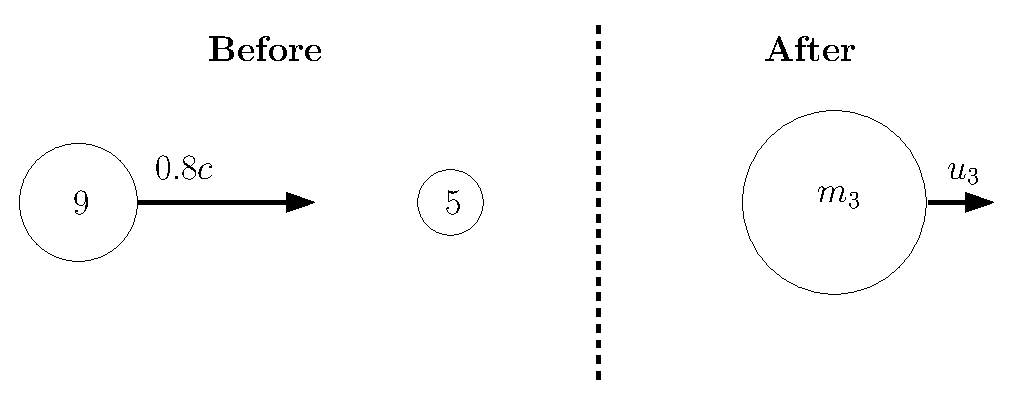
\includegraphics[width=3.8in]{relativistic_momentum_and_energy/relpande1.eps}
\end{center}
\caption{Collision discussed in Example \ref{ex:momentum-goodbye}.
\label{fig:momentum_goodbye}}
\end{figure}
\solution
The classical laws Eqs.~(\ref{eq:pcons}) and (\ref{eq:mcons}) would
yield
\begin{eqnarray}
\text{Eq.~(\ref{eq:pcons})}&\Rightarrow& 9\units{MeV/$c^2$}\times 0.8c + 
                     5\units{MeV/$c^2$}\times 0 = m_3u_3 \nonumber \\
                 &\Rightarrow& u_3 = \frac{7.2\units{MeV/$c$}}
                            {14\units{MeV/$c^2$}} = 0.514c\nonumber
\end{eqnarray}
and 

\begin{eqnarray}
\text{Eq.~(\ref{eq:mcons})}
&\Rightarrow& 9\units{MeV/$c^2$} + 
                     5\units{MeV/$c^2$} = m_3 \nonumber \\
                    &\Rightarrow& m_3 = 14\units{MeV/$c^2$}. \nonumber
\end{eqnarray}

Transform now to a frame in which the final particle is at rest.  This
clearly means that we should view the collision from a spaceship
traveling with particle 3 at $0.514c$ to the right, relative to the
original observer. Equation~(\ref{eq:vtransform-inverse}) gives
\begin{eqnarray}
u_3^\prime &=& \frac{u_3 - v}{1 - u_3v/c^2} = 
              \frac{0.514c - 0.514c}{1-0.514^2} = 0 \nonumber \\
u_5^\prime &=& \frac{u_5 - v}{1 - u_5v/c^2} = 
              \frac{0-0.514c}{1-0\times 0.514} = -0.514c \nonumber \\
u_9^\prime &=& \frac{u_9 - v}{1 - u_9v/c^2} = 
              \frac{0.8c - 0.514c}{1-0.8\times0.514} = 0.486c \nonumber
\end{eqnarray}
\begin{figure}[tb]
\begin{center}
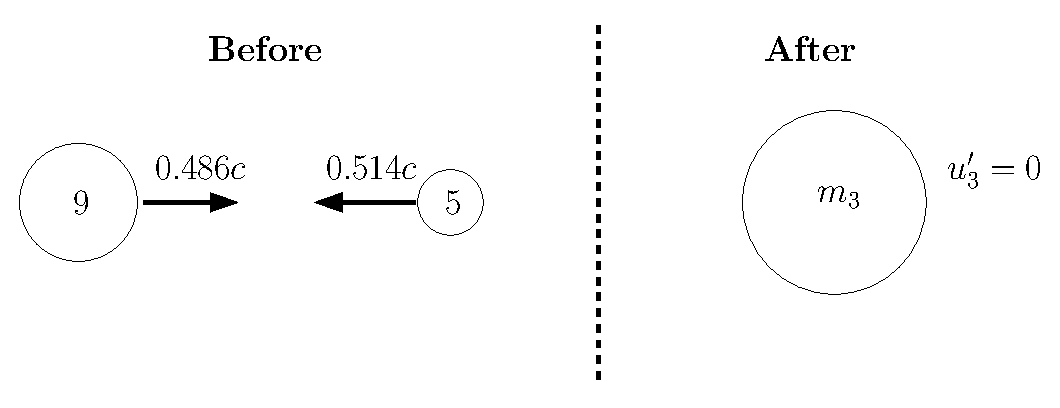
\includegraphics[width=3.8in]{relativistic_momentum_and_energy/relpande2.eps}
\end{center}
\caption{Collision discussed in Example \ref{ex:momentum-goodbye} as
viewed from rest frame of product particle.}
\label{fig:momentum_goodbyeII}
\end{figure}
In the new primed frame, the collision appears as in
Fig.~\ref{fig:momentum_goodbyeII}.  Checking the classical momentum
conservation law in the new frame gives
\begin{equation}
9\units{MeV/$c^2$}\times 0.486c + 5\units{MeV/$c^2$}\times (-0.514c) = 
   m_3 \times 0.
\end{equation}
But the left side of this equation here works out to be
$1.80\units{MeV/$c$}$ which is NOT equal to the right side (which is
0).  So, classical momentum is not conserved in this new frame.
Therefore, either (a) conservation of momentum isn't a valid law of
physics; (b) the Relativity Principle (invariance of the laws of
physics) is violated; or (c) we need a new definition for momentum.
\end{example}

You probably won't be surprised to hear that Einstein wasn't about to
give up on the Relativity Principle because of this argument.  After
all, he had already redefined time and space to make the Principle
work.  And although the classical expression for momentum does not lead to
invariance for high velocity collisions, there are attributes of
particles involving their masses and velocities that do produce
invariant conservation laws.  These quantities are called relativistic
momentum and relativistic energy, or more simply, momentum and energy.
They are defined by

\boxiteq{
\begin{equation}
\vec{p} = \frac{m\vec{u}}{\sqrt{1-u^2/c^2}} 
        \text{\hspace{0.2in}{\bf Definition of relativistic momentum}},
\label{eq:rel-p-def}
\end{equation}}

and

\boxiteq{
\begin{equation}
E = \frac{mc^2}{\sqrt{1-u^2/c^2}} 
\text{\hspace{0.2in}{\bf Definition of relativistic energy}}.
\label{eq:rel-e-def}
\end{equation}}

Einstein was motivated to define momentum and energy in this way
because conservation of momentum and energy defined in this
new way are invariant, as we will show with an example below.  Of
course, motivation is all very nice, but the most compelling reason
that the momentum and energy of a particle must be defined this way
instead of in the classical way is because experiments with high-speed
particles it is these new relativistic quantities that are conserved,
and not those given by the classical definitions.

Let's explore this invariance by redoing Example \ref{ex:momentum-goodbye} 
using Einstein's new definitions and the relativistic conservation laws:
\begin{equation}
\vec{p}_{\rm before} = \vec{p}_{\rm after}
\end{equation}
\begin{equation}
E_{\rm before} = E_{\rm after}
\label{eq:econs}
\end{equation}


\begin{example}{}
\label{ex:pe-cons}
Figure \ref{fig:junk} shows a particle of mass $9\units{MeV/$c^2$}$ and 
speed $0.8c$ striking a stationary particle of mass $5\units{MeV/$c^2$}$, 
producing a single particle of mass $16\units{MeV/$c^2$}$.
You might not be too happy here with the final particle having a mass
of $16\units{MeV/$c^2$}$, but hold on a little longer --- we'll
explain this shortly.  (A little preview --- this might be a good time
to take a pen and scribble Eq.~(\ref{eq:mcons}) out of existence.)  In
the next chapter, we'll learn more rigorously how to determine the
correct attributes of the final particle.  Here we just want to check
the conservation laws. (a) Check the conservation of relativistic
momentum and relativistic energy in the rest frame of the 
$5\units{MeV/$c^2$}$ particle.  (b) Check the conservation of
relativistic momentum and relativistic energy in the rest frame of the
$16\units{MeV/$c^2$}$ particle.
\begin{figure}[tb]
\begin{center}
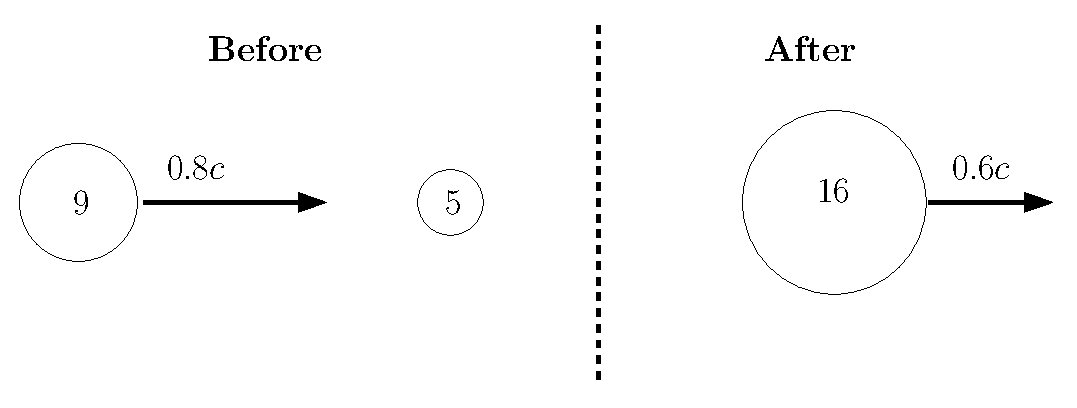
\includegraphics[width=3.8in]{relativistic_momentum_and_energy/relpande3.eps}
\end{center}
\caption{Collision discussed in Example \ref{ex:pe-cons}.}
\label{fig:junk}
\end{figure}

\solution
(a) We will use the relativistic definitions and conservation laws given 
in Eqs.~(\ref{eq:rel-p-def})--(\ref{eq:econs}).  Conservation of momentum 
gives 
\begin{equation}
\frac{9\units{MeV/$c^2$}\times 0.8c}{\sqrt{1 - 0.8^2}} + 0 = 
\frac{16\units{MeV/$c^2$}\times 0.6c}{\sqrt{1 - 0.6^2}},
\end{equation}
and conservation of energy gives
\begin{equation}
\frac{9\units{MeV/$c^2$}\times c^2}{\sqrt{1 - 0.8^2}} 
 + \frac{5\units{MeV/$c^2$}\times c^2}{\sqrt{1 - 0^2}}= 
\frac{16\units{MeV/$c^2$}\times c^2}{\sqrt{1 - 0.6^2}}.
\end{equation}
The momentum equation gives $12\units{MeV/$c$} = 12\units{MeV/$c$}$, 
while the energy equation gives $15\units{MeV} + 5\units{MeV} = 20\units{MeV}$.
So the conservation laws are satisfied in this frame.

(b) Now, transform to a frame in which the final particle is at rest, by
viewing from a spaceship moving at $0.6c$ to the right.  The velocity
transformations give
\begin{eqnarray}
u_{16}^\prime &=& \frac{u_{16}-v}{1 - u_{16}v/c^2} 
   = \frac{0.6c -0.6 c}{1-0.6^2} = 0 \\
u_{5}^\prime &=& \frac{u_{5}-v}{1 - u_{5}v/c^2} 
   = \frac{0 -0.6 c}{1-0\times 0.6} = -0.6c = -\frac{3}{5}c \\
u_{9}^\prime &=& \frac{u_{9}-v}{1 - u_{9}v/c^2} 
   = \frac{0.8c -0.6 c}{1-0.8\times 0.6} = \frac{5}{13}c \simeq 0.385c 
\end{eqnarray}
\begin{figure}[b]
\begin{center}
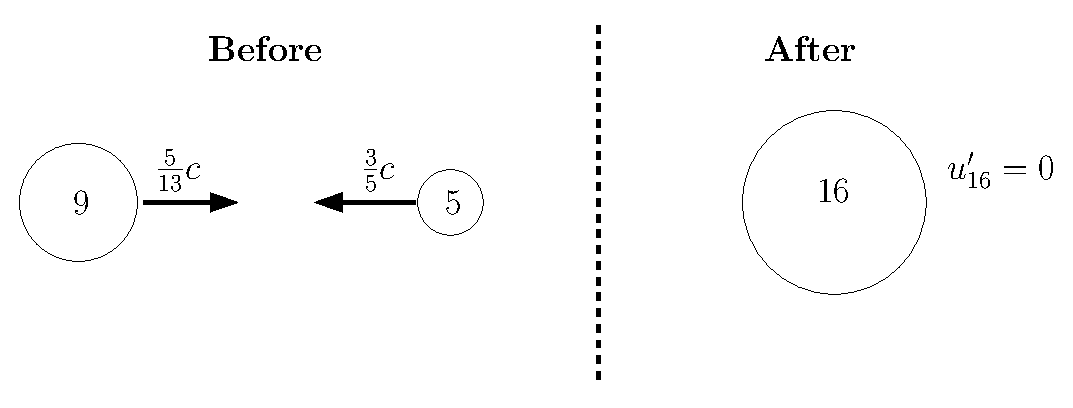
\includegraphics[width=3.8in]{relativistic_momentum_and_energy/relpande4.eps}
\end{center}
\caption{Collision discussed in Example \ref{ex:pe-cons} as viewed from 
rest frame 
of product particle.}
\label{fig:junk2}
\end{figure}
In this new frame, the collision appears as in Fig.~\ref{fig:junk2}.
When we check the relativistic conservation laws in this new frame, we find: 
\begin{equation}
\frac{9\units{MeV/$c^2$}\times 5c/13}{\sqrt{1 - (5/13)^2}} 
    -  \frac{5\units{MeV/$c^2$}\times 3c/5}{\sqrt{1 - (3/5)^2}}= 
\frac{16\units{MeV/$c^2$}\times 0}{\sqrt{1 - 0^2}}
\end{equation}
\begin{equation}
\frac{9\units{MeV/$c^2$}\times c^2}{\sqrt{1 - (5/13)^2}} 
 + \frac{5\units{MeV/$c^2$}\times c^2}{\sqrt{1 - (3/5)^2}}= 
\frac{16\units{MeV/$c^2$}\times c^2}{\sqrt{1 - 0^2}}
\end{equation}
The momentum equation gives
\begin{equation}
\frac{15}{4}\units{MeV/$c$} -\frac{15}{4}\units{MeV/$c$} = 0,
\end{equation}
which checks out, while the energy equation gives
\begin{equation}
\frac{39}{4}\units{MeV} +\frac{25}{4}\units{MeV} = 16\units{MeV}
\end{equation}
which also checks out.  This means the conservation laws are true in
both the original and the new frame, and the Relativity Principle is
upheld with Einstein's new definitions.
\end{example}


This may be a nice argument on paper, but does it work in practice?
Are relativistic momentum and energy, rather than classical momentum
and mass, really conserved in particle interactions?  The answer is an
emphatic {\bf YES}!  In countless interactions observed in high-energy
particle accelerators, relativistic momentum and energy are always
found to be conserved.

\section{Another Invariant}

We now have relativistic expressions for energy and momentum.
It turns out that these can be combined to form an invariant, just
like we combined distance and time to get the invariant spacetime
interval.  Recall from chapter 4, we defined the square of the
interval as
\begin{equation}
I^2 = \left(c\Delta t\right)^2 - \left(\Delta x\right)^2.
\end{equation}
We can combine energy and momentum of an object or particle in a
similar manner to get an invariant:
\begin{equation}
m^2 = \left(\frac{E}{c^2}\right)^2 - \left(\frac{p}{c}\right)^2.
\label{eq:m-invariance1}
\end{equation}
Given any object or particle with energy $E$ and momentum $p$ as
measured by an observer in a reference frame, this observer can easily
calculate the value of $m$ for that object.  If a different observer is
in another reference frame (labeled with ``primes") and determines 
$E^\prime$ and $p^\prime$ for the same particle, she will find that 
if she calculates
\begin{equation}
\left(m^\prime\right)^2 = \left(\frac{E^\prime}{c^2}\right)^2 
          - \left(\frac{p^\prime}{c}\right)^2,
\end{equation}
then she will get exactly the same value for $m^\prime$  that the first
observer found for $m$.  In other words
\begin{equation}
m=m^\prime,
\end{equation}
or
\begin{equation}
E^2 - (pc)^2 = \left(E^\prime\right)^2 - \left(p^\prime c\right)^2.
\label{eq:m-invariance2}
\end{equation}
In the same manner that we used the invariant spacetime interval to
relate $\Delta x$ and $\Delta t$ as measured in one reference frame to 
$\Delta x^\prime$ and $\Delta t^\prime$ in
another reference frame, we can use the invariance of $m$ to relate $E$
and $p$ in one frame to $E^\prime$ and $p^\prime$ in a different frame.

What is this invariant $m$?  This is simply the mass of the object.
In words, the invariance expressed in
Eqs.~(\ref{eq:m-invariance1}--\ref{eq:m-invariance2}) states that
all observers agree about the mass of an object.\footnote{You may hear
people saying that in relativity, ``a person's mass increases as (s)he
approaches the speed of light.''  (In fact, it used to be common for
physicists to say this.)  This is an unfortunate claim.  What they are
doing is saying, ``Well, since $p = mu/\sqrt{1-u^2/c^2}$, we're going
to artificially call $m/\sqrt{1-u^2/c^2}$ the relativistic mass so
that we can hold on to the $p=mu$ definition of momentum.''  There is
no reason to do this --- there is nothing in relativity that requires
us to redefine mass and, in fact, mass is an invariant.}

We can rewrite Eq.~(\ref{eq:m-invariance1}) in a slightly more
convenient form
\begin{equation}
E^2 - (pc)^2 = (mc^2)^2.
\label{eq:m-invariance3}
\end{equation}
As we'll see in the next chapter, this is actually the most useful of
all the energy and momentum relations.  It applies to {\em every}
particle in {\em every} situation.  (We'll see that
Eqs.~(\ref{eq:rel-p-def}) and (\ref{eq:rel-e-def}) aren't very useful
for `particles' of light.)  In the homework for tonight, you'll show
that this relation comes very easily from the relativistic definitions
for energy and momentum (\ref{eq:rel-p-def}) and (\ref{eq:rel-e-def}).


\section{Rest Energy and Kinetic Energy}
Let's look more closely at what we called the relativistic energy of a
particle in Eq.~(\ref{eq:rel-e-def}).  If the particle is at rest, so
that $u = 0$, the energy reduces to $E = mc^2$, perhaps the most famous
formula in all of physics.  So we discover that a particle has energy
even when it's not moving!  This energy is called the {\em rest energy}, 
$E_0$.  That is
\begin{equation}
E_0 = mc^2.
\label{eq:emc2}
\end{equation}
This is a remarkable result! Consider an apple with a mass of 
$100\units{g}=0.1\units{kg}$.    Einstein
says that this apple has an energy at rest of $E_0 = 
0.1\units{kg}\times (3\times 10^8)^2 = 9\times 10^{15}\units{J}$!
This is a huge amount of energy. Let's compare this to a classical 
energy.

You know that the classical kinetic energy of a particle is 
$K_{\rm class.}  = \frac{1}{2}mv^2$.  For the $0.1\units{kg}$ 
apple falling at $10\units{m/s}$ we get $K_{\rm class.} = 5\units{J}$.  
This is the energy that the apple has because it is in motion.
In relativistic physics, kinetic energy is not expressed as 
$K = \frac{1}{2}mv^2$,  but it is still defined as the energy that 
a particle has {\em because it is in motion}.  The relativistic 
kinetic energy is the difference between a particle's energy when 
it is moving and its rest energy, 
\begin{equation}
K = E - mc^2 = \frac{mc^2}{\sqrt{1-u^2/c^2}} - mc^2.
\label{eq:rel-k-def}
\end{equation}
This doesn't resemble the classical expression for kinetic
energy $K_{\rm class.} = \frac{1}{2}mv^2$ (or, since we
use $v$ for the velocity of the frame and $u$ as the velocity of the
particle, $K = \frac{1}{2}mu^2$).  Since we know that the classical
expression for kinetic energy is valid in the low-speed regime, the
relativistic kinetic energy given be Eq.~(\ref{eq:rel-k-def}) must
somehow reduce to the classical expression when the speed of the
particle is small compared to the speed of light.  We show the
connection between the relativistic and classical forms of kinetic
energy in the next example.

The relativistic expressions for energy and kinetic energy have 
amazing consequences.  In collisions of high speed particles, or 
in radioactive decays, it is the total energy of a system of 
particles that is conserved, not the mass.  In these processes,
rest energy ($mc^2$) can be converted into kinetic energy, and vice 
versa.  In a decay, the loss of a small amount of mass corresponds to the 
loss of a huge amount of rest energy, which will be manifested 
in a huge increase in kinetic energy. 
 
 


%However, this doesn't resemble the classical expression for kinetic
%energy, which as you recall was $K = \frac{1}{2}mv^2$ (or, since we
%use $v$ for the velocity of the frame and $u$ as the velocity of the
%particle, $K = \frac{1}{2}mu^2$.).  Since we know that the classical
%expression for kinetic energy is valid in the low speed regime, the
%relativistic kinetic energy given be Eq.~(\ref{eq:rel-k-def}) must
%somehow reduce to the classical expression when the speed of the
%particle is small compared to the speed of light.  We show the
%connection between the relativistic and classical forms of kinetic
%energy in the next example.



% --- the implications are two-fold: first,
%the relation implies that matter and energy aren't separate
%quantities, but are really just different forms of the same thing; and
%second, implied in this relation is the possibility of converting
%between matter and energy.  {\em And the conversion factor is $c^2$
%--- a huge number (when expressed in ``everyday'' units of m$^2$/s$^2$
%or J/kg)!}  To get an idea of the magnitude of this factor, try
%computing the amount of energy contained in a 1 gm paper clip.
%    
%You know from classical physics that the energy associated with a
%particle's motion is called kinetic energy.  However in relativistic
%physics, kinetic energy is not expressed as $K = \frac{1}{2}mv^2$.
%Instead, it is defined as the difference between a particle's energy
%when it is moving and its rest energy,
%\begin{equation}
%K = E - mc^2 = \frac{mc^2}{\sqrt{1-u^2/c^2}} - mc^2.
%\label{eq:rel-k-def}
%\end{equation}
%However, this doesn't resemble the classical expression for kinetic
%energy, which as you recall was $K = \frac{1}{2}mv^2$ (or, since we
%use $v$ for the velocity of the frame and $u$ as the velocity of the
%particle, $K = \frac{1}{2}mu^2$.).  Since we know that the classical
%expression for kinetic energy is valid in the low speed regime, the
%relativistic kinetic energy given be Eq.~(\ref{eq:rel-k-def}) must
%somehow reduce to the classical expression when the speed of the
%particle is small compared to the speed of light.  We show the
%connection between the relativistic and classical forms of kinetic
%energy in the next example.

\begin{example}{Relating relativistic and classical expressions 
for kinetic energy}  

Use the binomial approximation in Eq.~(\ref{eq:rel-k-def}) to find
an approximate expression for $K$ when $u$ is much smaller than
$c$, i.e., when $u/c \ll 1$.  (The binomial expansion states that
$(1-\epsilon)^{-1/2} \simeq 1 + \frac{1}{2}\epsilon + \cdots$ if
$\epsilon$ is small.)

\solution
We write $1/\sqrt{1-u^2/c^2}$ as $(1 - u^2/c^2)^{-1/2}$ so that
Eq.~(\ref{eq:rel-k-def}) becomes
\begin{eqnarray}
K &=& mc^2\left(1-u^2/c^2\right)^{-1/2} - mc^2 \nonumber \\
  &=& mc^2 \left(1 + \frac{1}{2}\frac{u^2}{c^2} + \cdots\right) - mc^2 \\
  &\simeq&  \frac{1}{2}mu^2 \nonumber, 
\end{eqnarray}
where in the last line we have assumed the classical limit in which
$u/c \ll 1$.
Thus we see that the classical expression for kinetic energy is only a
low-velocity approximation to the correct expression, given by
Eq.~(\ref{eq:rel-k-def}).
\end{example}

\section{Photons: Particles with Zero Mass}

How do we deal with the energy and momentum of light? As you will see
next semester in PHYS 212, the same year that Einstein published his
first paper on Special Relativity, he also proposed that light must be
considered to be composed of particles which are now called photons.
(This was the first of the three 1905 papers that we discussed at the
beginning of Chapter \ref{chapter:relativityI}.)  Since light always travels
at a speed $c$ in a vacuum, then photons in a vacuum must travel at
that speed regardless of the reference frame of the observer.  But if
we look back at Eqs.~(\ref{eq:rel-p-def}) and (\ref{eq:rel-e-def}), we
find that the denominators of both equations are zero for a particle
moving at the speed of light, and clearly a photon cannot have
infinite momentum or infinite energy.

    
The only way to resolve this dilemma is to postulate that photons are
particles with zero mass ($m = 0$).  Equations~(\ref{eq:rel-p-def})
and (\ref{eq:rel-e-def}) are still not very useful in this case, since a
fraction which has zero in both the numerator and denominator is
undefined.  However, with zero mass these equations no longer imply 
infinite energy and momentum for particles moving at light speed.
    
For a massless particle (such as photons),
Eq.~(\ref{eq:m-invariance3}) can be rewritten for $m=0$ as
\begin{equation}
E = \vert p\vert c\text{\hspace{0.25in}{\bf for massless particles only.}}
\label{eq:e-photon}
\end{equation}
Remember, Eq.~(\ref{eq:e-photon}) is valid only for massless
particles.

\section{More experimental evidence}

Now that we have introduced the relativistic relations for energy and
momentum, we can discuss some additional pieces of evidence that
Einstein's theory of relativity is, in fact, correct.  The following
examples can be added to those presented in Chapter
\ref{chapter:relativityI}.  Remember that if even one of these
experiments had disagreed with Einstein's theory, then the entire
theory would have to be thrown out since everything is internally
consistent.
\begin{itemize}
\item {\bf Particle accelerators}. As we already discussed in
Chapter~\ref{chapter:relativityI}, subatomic particles are frequently
accelerated in high energy experiments to speeds very close to $c$,
but no one has ever managed to accelerate a particle with mass to a
speed greater than $c$.  There's more here, though: as the particle's
speed (relative to the laboratory) gets closer and closer to $c$, the
amount of energy that has to be added to increase the speed further
gets larger and larger, diverging as the speed approach $c$.  For
instance, the amount of energy that needs to be added to accelerate a
particle from $0.98c$ to $0.99c$ has been found experimentally to be much
larger than the energy to accelerate the same particle from $0.97c$ to
$0.98c$, and in fact, much larger than that predicted classically.  As
is the case with all other tests of relativity, the amount of energy
to be added agrees perfectly with Einstein's predictions.  Homework
problem \ref{prob:energy-to-accelerate}  investigates this further.
\item {\bf Collisions of high-energy particles}.  When subatomic
particles are slammed into each other with high energies, new
particles are actually created that weren't there before the
collision.  These collisions are converting kinetic energy (KE) into
matter, and this is done all the time in particle accelerators.  (This
is, in fact, the main tool that physicists use to study massive
subatomic particles.)  This is an experimental result that simply
cannot be explained classically.  Once again, though, the results
agree perfectly with Einstein's theory.  We will be discussing this in
more detail in Chapter \ref{chapter:relativity_app}, and you will be doing
(or have already done) a lab on this (the Relativistic Energy and
Momentum lab).
\item {\bf Matter-to-KE conversions}.  One of the most convincing and
most dramatic tests of Einstein's theory of relativity occurred on
July 16, 1945, in New Mexico when the first atomic bomb was exploded,
converting matter into a horrifying amount of kinetic energy (don't
forget that factor of $c^2$ in the famous $E = mc^2$ equation).  Since
then, there have been quite a few additional such demonstrations of
Einstein's theory.  (And again, the quantitative aspects of these
demonstrations agree perfectly with the theory.)
    
It isn't necessary to explode a bomb to convert matter into energy.
Nuclear energy has found peaceful applications in the area of power
generation. (There is a nuclear power plant in Berwick, PA, in fact,
which you can see easily if you drive on Rt.~80 toward New Jersey,
shortly after passing Bloomsburg).  We will discuss nuclear power
generation more in the next chapter (including fusion power ---  still
being developed --- which doesn't produce any long-lasting radioactive
waste).

\end{itemize}

\section{A note on units}
\label{section:rel-units}

When working with energy and momentum for small, subatomic particles
(the ones that are most typically traveling at relativistic speeds),
it is convenient to define a unit of energy called the ``electron
volt'' (eV for short).  One electron volt is the kinetic energy gained
by an electron when accelerated through a 1 volt potential difference.
(You'll learn more about this in PHYS 212.)  Quantitatively, $1\units{eV} =
1.6\times 10^{-19}\units{J}$.  An analogous energy unit might be a
``superball-meter'' --- the amount of kinetic energy gained by a
superball when dropped 1 m.
    
For high energy particles, the energies can get into the thousands,
millions or billions of electron volts, so we also define 
$1\units{keV} = 10^3\units{eV}$, $1\units{MeV} = 10^6\units{eV}$,
$1\units{GeV} = 10^9\units{eV}$.
    
Units for mass and momentum are also defined in terms of energy in
relativity.  For mass, we use eV/$c^2$ --- ``electron volts per
$c^2$'' --- or keV/$c^2$, MeV/$c^2$, GeV/$c^2$.  For momentum, we use
eV/$c$ (or keV/$c$, MeV/$c$, GeV/$c$).  For example, an electron has a
mass of $511\units{keV/$c^2$}$; conceptually, this means that an electron 
has a rest energy of $511\units{keV}$, or that its mass --- if converted 
completely into kinetic energy --- would produce $511\units{keV}$ of 
kinetic energy.
  
{\bf Warning}: when using these units, don't throw any numbers in for
the $c$ --- it is part of the unit.  So, the mass of an electron
should be written as ``$511\units{keV/$c^2$}$'' (or $0.511\units{MeV/$c^2$}$), 
{\bf not} as $511\units{keV}/(3.0\times 10^8\units{m/s})^2$ \hspace{-1.7in}\rule[1mm]{42mm}{.2mm} 
or $511\units{keV}/(1\units{lt-s/s})^2$.\hspace{-1.25in}\rule[1mm]{30mm}{.2mm}
\newpage

\section{Summary}
The various equations introduced in this chapter are summarized as
in Table \ref{table:rel-defs}.

\begin{table}[h]
\begin{small}
\caption{Relativistic formulas for energy and momentum.}
\label{table:rel-defs}
\begin{tabular}{|lclc|} \hline
\parbox{3.0cm}{\raggedright{\bf Definition of momentum:}}   &  
       \parbox{3.cm}{\[ \vec p =\frac{m\vec u}{\sqrt{1-u^2/c^2}} \]} & 
\parbox{3.0cm}{\raggedright{\bf Definition of energy:}} & 
       \parbox{3.cm}{\[ E =\frac{mc^2}{\sqrt{1-u^2/c^2}} \]} \\
\parbox{3.0cm}{\raggedright {\bf Energy in terms of momentum and mass:}}   &  
       \parbox{3.cm}{\[ E^2 = p^2c^2 + m^2c^4\]} & 
\parbox{3.0cm}{\raggedright{\bf Velocity in terms of energy and momentum:}\\
       (See Problem \arabic{chapter}.\ref{prob:rel-u-p-e}.)} & 
       \parbox{3.cm}{\[ \vec{u} = \frac{\vec{p}c^2}{E} \]} \\
       & & & \\
\parbox{3.0cm}{\raggedright{\bf Definition of kinetic energy:}}   &  
       \parbox{3.cm}{\[ K = E - mc^2 \]} & 
\parbox{3.0cm}{\raggedright{\bf Energy in terms of momentum for 
zero-mass particle:}} & 
       \parbox{3.cm}{\[ E = \left|\vec{p}\right|c \]} \\
&  & & \\ \hline
\end{tabular}
\end{small}
\end{table}

\newpage

\section*{Problems}
\markright{PROBLEMS}

\begin{problem}
Duck Dodgers hops in his spaceship and leaves the Earth at a
speed $0.6c$ in an attempt to reach the newly discovered Planet X before
aliens from Mars.
    \begin{enumerate}
    \item Mission control on Earth sends an encoded message (a
    flashing beacon) to Duck Dodgers warning him about the progress of
    the Martian ship.  The light pulses travel at a speed $c$ relative
    to observers on the Earth.  How fast are the pulses traveling
    relative to Duck Dodgers?
    \item Duck Dodgers doesn't understand the message that he
    received, so he sends a radio message back toward the Earth asking
    for clarification.  The radio signal is traveling at a speed $c$
    relative to the Duck.  How fast is the signal traveling relative
    to observers on the Earth?
    \item The radio message is intercepted by the Martian who is
    behind Duck Dodgers but traveling in the same direction at a speed
    $0.8c$ relative to the Earth.  How fast is the radio message going
    relative to the Martian?
    \item The radio message is also intercepted by one of the
    Martian's monsters who is traveling back toward the Earth to
    attack.  The monster is traveling at a speed $0.9c$ relative to the
    Martian.  How fast is the radio signal relative to the monster?
    \end{enumerate}
\end{problem}

\begin{problem}
A particle travels at speed $0.50c$ relative to Captain Kirk.
Mr.\ Spock is traveling at a speed $0.70c$ relative to Captain Kirk,
in the same direction as the particle.
Calculate the velocity of the particle relative to Mr.\ Spock.
\label{prob:vtransform}
\end{problem}

\begin{problem}
A proton's velocity is measured at $0.6c$ relative to an observer
on earth, and $0.8c$ relative to an observer passing by in a rocket.
Determine the speed of the rocket relative to earth.  (There 
are two possible correct answers that correspond to two different
physical situations.)
\label{prob:vtransform2}
\end{problem}

\begin{problem}
After traveling on vacation to Betelgeuse to witness a supernova, Fred
and Ethel are returning home, traveling at a speed $0.75c$ relative to
and toward the Earth.  Ethel is particularly anxious to get home and
see her new great-great-great-great-great-great-great-great grandson,
so she hops on the emergency shuttlecraft, which leaves Fred's ship
traveling at a speed of $0.75c$, relative to Fred.  How fast is Ethel's
shuttle traveling relative to the Earth?
\end{problem}

\newpage
\begin{problem}
A particle of mass $3m$, moving at speed $0.60c$ in the positive
$x$-direction, collides with and sticks to a particle of mass $2m$
originally at rest.  Assume a head-on collision.
\begin{enumerate}
\item Calculate the initial total momentum before impact, using the
classical definition, $p = mu$, for momentum. 
\item Assuming conservation of mass as well as classical momentum,
find the velocity of the composite particle of mass $5m$ after the
collision.  
\item Now transform to a primed frame in which the particle of mass
$3m$ is at rest.  Use the relativistic velocity transformation to
compute the velocities $u^\prime_{3m}$, $u^\prime_{2m}$, and
$u^\prime_{5m}$ in the primed frame. 
\item Still in the primed frame, check whether momentum $mu^\prime$ is
conserved by computing the total momentum before the collision and the
total momentum after the collision.
\end{enumerate}
\label{prob:inelastic}
\end{problem}


\begin{problem}
Show that the velocity of a particle expressed in terms of
relativistic energy and momentum is $u = pc^2/E$.
\label{prob:rel-u-p-e}
\end{problem}


\begin{problem}
An electron is accelerated from a velocity $u_1 = 0.98c$ to a velocity
$u_2 = 0.99c$.  Calculate the change in the electron's kinetic energy in
units of MeV.  ($m_{\rm electron} = 0.511\units{MeV/$c^2$}$.)
\label{prob:energy-to-accelerate}
\end{problem}

\begin{problem}
Electron A has a total energy of $1.0\units{MeV}$.  Electron B has a
kinetic energy of $0.25\units{MeV}$.  Electron C has a kinetic energy of
$0.75\units{MeV}$.  Electron D has a momentum of $1.0\units{MeV/$c$}$.
For each of the electrons A through D, determine its energy, momentum,
kinetic energy, and speed.
\label{prob:electrons}
\end{problem}

\begin{problem}
A certain particle has a total energy of $1.20\units{MeV}$ and
a momentum of $0.95\units{MeV/$c$}$.  Calculate the particle's mass,
kinetic energy, and velocity.  
\end{problem}

\begin{problem}
Compute the momentum and velocity of a proton that has a total
energy equal to 7 times its rest energy.  ($m_{\rm proton} =
938\units{MeV/$c^2$}$.)
\label{prob:proton}
\end{problem}

\begin{problem}
Combine Eqs.~(\ref{eq:rel-p-def}) and (\ref{eq:rel-e-def}) to derive 
Eq.~(\ref{eq:m-invariance3}).
\end{problem}

\begin{problem}
Show, from Eq.~(\ref{eq:m-invariance3}) and the result of
problem (\ref{prob:rel-u-p-e}) that any massless particle moves at
the speed of light and that if a particle moves at the speed of light
it must have zero mass.    
\end{problem}

\begin{problem}
A proton (mass $938\units{MeV/$c^2$}$) is traveling at velocity
$0.60c$ in the $+x$ direction relative to a spaceship which itself is
traveling at velocity $0.80c$ in the $+x$ direction relative to Earth.
Calculate the velocity and then the energy and momentum of the proton
as measured in the Earth frame.
\end{problem}

\begin{problem}
A particle's energy and momentum in one frame are $41\units{MeV}$ and 
$40\units{MeV/$c$}$ respectively.  Find the particle's energy and 
momentum as measured in a different frame in which the particle's speed is 
$u^\prime = 0.8c$.
\label{prob:ep_transform}    
\end{problem}

\begin{problem}
Given a particle with $E_A = 21\units{MeV}$ and $p_A
= 15\units{MeV/$c$}$ as measured in reference frame {\bf A}, and 
$E_B = 20\units{MeV}$ as measured in frame {\bf B}, determine the 
mass $m_B$ and momentum $p_B$ of the particle as measured in 
frame {\bf B}.  
\end{problem}

\begin{problem}
The Fermi National Accelerator Laboratory (Fermilab) is located outside
Chicago, Illinois, and is one of the world's largest particle accelerator
facilities.  At Fermilab, protons (mass $938\units{MeV/$c^2$}$) are given
huge amounts of energy and achieve velocities that are nearly the speed
of light.
\begin{enumerate}
\item Prior to a recent upgrade, protons at Fermilab could reach
speeds that were only $163\units{m/s}$ slower than the speed of
light.  How much energy is required to get a proton from rest up to
the speed $u = c - 163\units{m/s}$?  
\item After the upgrade, the protons were able to reach the speed $u
=c - 132\units{m/s}$ (a whopping increase of $31\units{m/s}$).
How much additional energy is required to get this $31\units{m/s}$
increase?
\item The Large Hadron Collider currently being developed at CERN (a
  particle accelerator facility in Europe) is designed to get protons
  up to an energy of $7.0\units{TeV}$. ($1\units{TeV} =
  10^{12}\units{eV}$).  Determine $u/c$, the ratio of the speed of the
  proton to the speed of light (note that $u/c$ is NOT equal to 1!)
\end{enumerate}
\label{prob:fermilab}
\end{problem}

\begin{problem}
A certain J-boson has mass of $150\units{MeV/$c^2$}$, speed of
$0.8c$, and total energy of $250\units{MeV}$.  Determine
the J-boson's momentum and kinetic energy.
\label{prob:J}
\end{problem}

\begin{problem}
A proton (mass $938\units{MeV/$c^2$}$) traveling down a beam pipe at
Fermilab is determined to have kinetic energy of $1.2\units{GeV}$.
Determine this proton's momentum and speed.
\label{prob:fermilab2}
\end{problem}
\newpage

\begin{problem}
An evil genius fires a rocket into a star, destroying the star.
Ten minutes later, as measured in the reference frame of the star,
debris thrown out from the explosion demolishes a
populated planet a distance $7\units{lt-min}$ from the star, as measured
in the star/planet frame.  Simultaneous with the explosion (according
to the star/planet reference frame), the Starship
Enterprise is $5\units{lt-min}$  from the star, on the opposite side from
the planet.  The Enterprise is
heading toward the star/planet system with a
speed of $0.6c$ relative to the planet and star.
\begin{enumerate}
     \item Draw a spacetime diagram for this situation.  Take the
       star/planet reference frame as the unprimed frame, and draw the
       world lines of the star and the planet, showing that they are
       $7\units{lt-min}$ apart.  Indicate the destruction of the star
       as event A on your spacetime diagram, and indicate the
       destruction of the planet as event B on your spacetime diagram.
       Also, draw the world line for the debris sent from the star to the
       planet.
     \item Draw the world line of the Starship Enterprise on your spacetime
     diagram, showing both the velocity of the spaceship and the correct
     location of the Enterprise when the star explodes.
    \item Calculate the speed of the matter thrown out from the explosion
     as measured by Starfleet officers on board the Enterprise.
     \item Calculate the time interval between the explosion of the star
     and the destruction of the planet, as measured by Starfleet officers
     on board the Enterprise.  (Hint:  use your result from (c) to
     determine an expression for the distance between events ---
     according to the Enterprise --- in terms of the unknown time between
     events.)
     \end{enumerate}
\label{prob:evil_genius}
\end{problem}
\newpage

\begin{problem}{\bf Are momentum and energy conserved?}\\
A mad scientist at rest in a lab on the earth is colliding particles together
to make more massive particles.  She creates head-on collisions of 
particles with a mass of $4\units{GeV/$c^2$}$ and speed $0.6c$ to create 
particles at rest with a mass of $10\units{GeV/$c^2$}$.

In the rest frame of the scientist, the  $4\units{GeV/$c^2$}$ particles
have equal and oppositely directed momenta, and the $10\units{GeV/$c^2$}$
particle is at rest, so momentum is conserved.

An observer in a rocket flying over the lab at a speed $v=0.6c$ views this 
experiment.  

\begin{enumerate}
\item Test whether {\bf relativistic} momentum is conserved 
according to the observer in the rocket.  Your test should include 
detailed numerical calculations  demonstrating the conservation 
(or non-conservation) of {\bf relativistic} momentum.
\item  Test whether {\bf relativistic} energy is conserved 
according to the scientist in her lab.  Your test should include 
detailed numerical calculations demonstrating the conservation 
(or non-conservation) of {\bf relativistic} energy.
\item  Test whether {\bf relativistic} energy is conserved 
according to the observer in the rocket.  Your test should include 
detailed numerical calculations demonstrating the conservation 
(or non-conservation) of {\bf relativistic} energy.
\end{enumerate}
 
 \begin{figure}[h]
    \begin{center}
    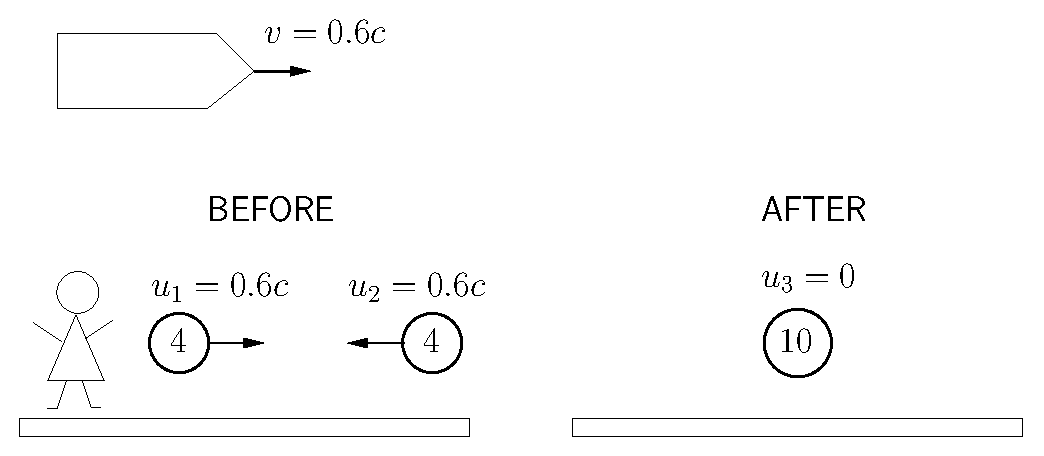
\includegraphics[width=4.25in]{relativistic_momentum_and_energy/atomsmasher.eps}
    \end{center}
    \caption{Figure for Problem \ref{prob:is_momentum_conserved}.}  
    \label{fig:is_momentum_conserved}
  \end{figure}

\label{prob:is_momentum_conserved}
\end{problem}
